The dijet invariant mass distribution for the sum of electron 
and muon events is shown after a fit of the sum of the Standard 
Model contributions to data in Figure~\ref{fig:CombinedFit}. 
Figure~\ref{fig:CombinedFitSubtracted} shows the distribution 
after subtraction of fitted background components obtained in 
Figure~\ref{fig:CombinedFit}.
Similar plots from separate fit to muon and electron data are shown in 
Figures~\ref{fig:MuFit}--\ref{fig:MuFitSubtracted} and 
Figures~\ref{fig:EleFit}--\ref{fig:EleFitSubtracted} 
respectively.
%%%%%%%%%%%%%%%%%%%%%%%%%%%%
%%%%%%%%%%%%%%%%%%%%%%%%%%%%
%%%%%%%
\begin{figure}[h!] {\centering
\unitlength=0.33\linewidth
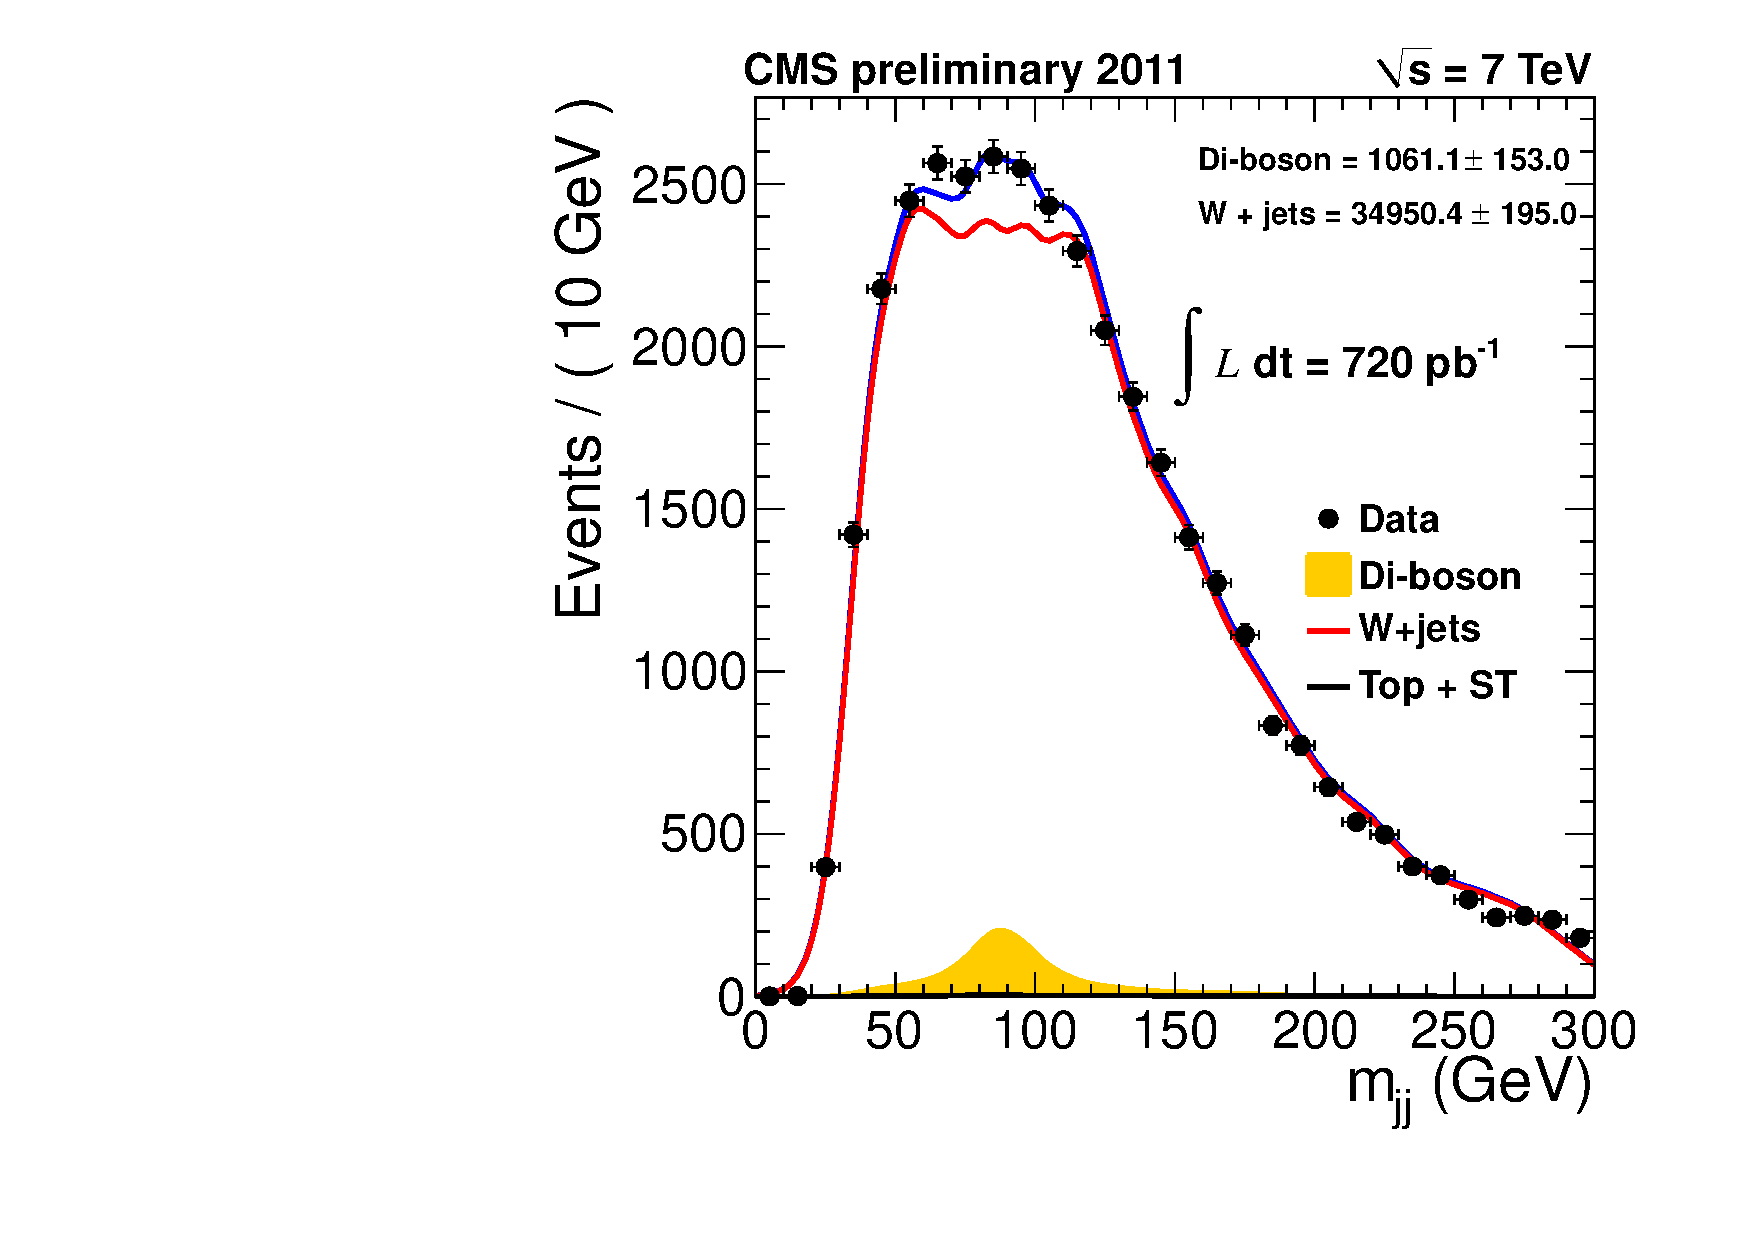
\includegraphics[width=0.48\textwidth]{figs/mJJ-combined-fit.pdf}
\put(-0.80,0.0){(a)} 
\unitlength=0.33\linewidth
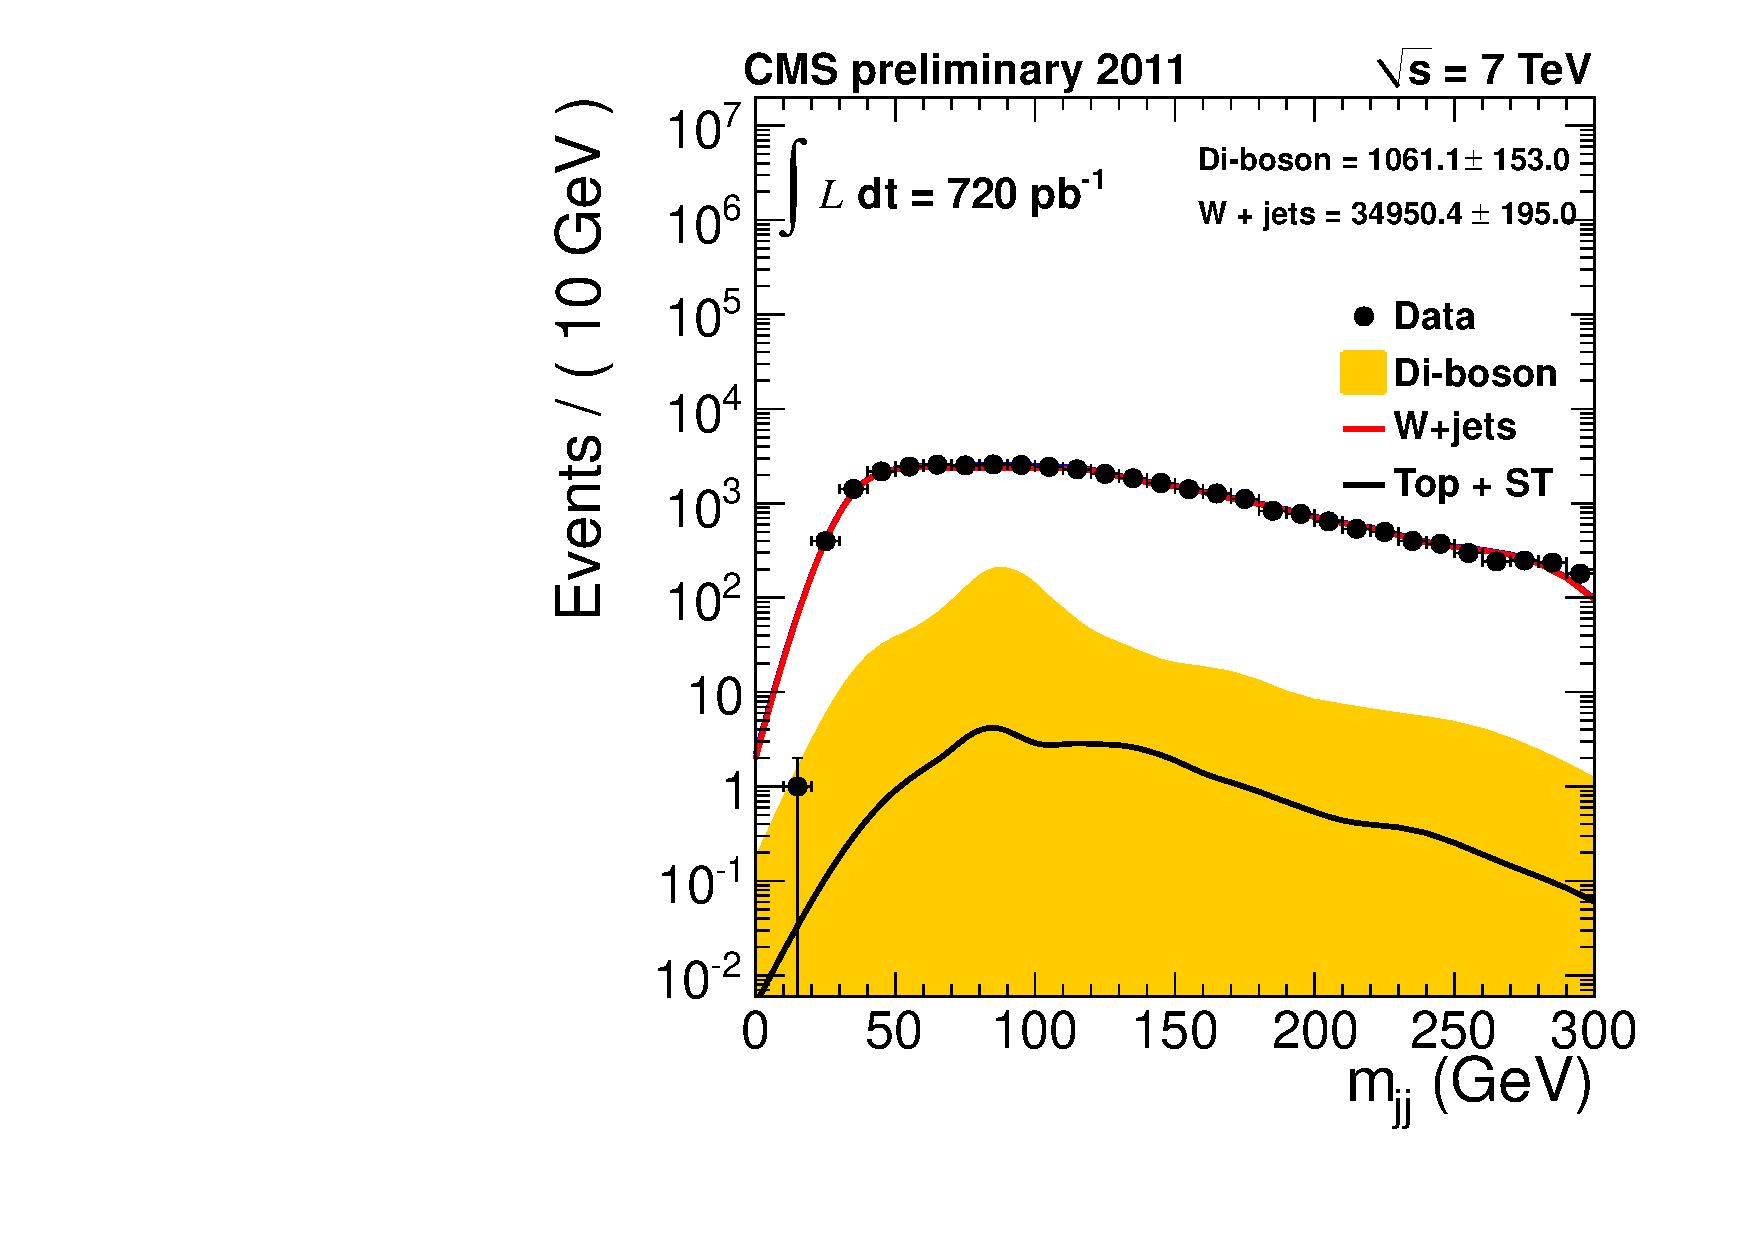
\includegraphics[width=0.48\textwidth]{figs/mJJ-combined-fit-logY.pdf}
\put(-0.80,0.0){(b)} 
\caption{
Projection of the $m_{jj}$ fit  to extract diboson signal for the sum 
of electron and muon events  (a) on linear scale and 
(b) on logarithmic scale.} 
\label{fig:CombinedFit}}
\end{figure}
%%%%%%%
%%%%%%%
\begin{figure}[h!] {\centering
    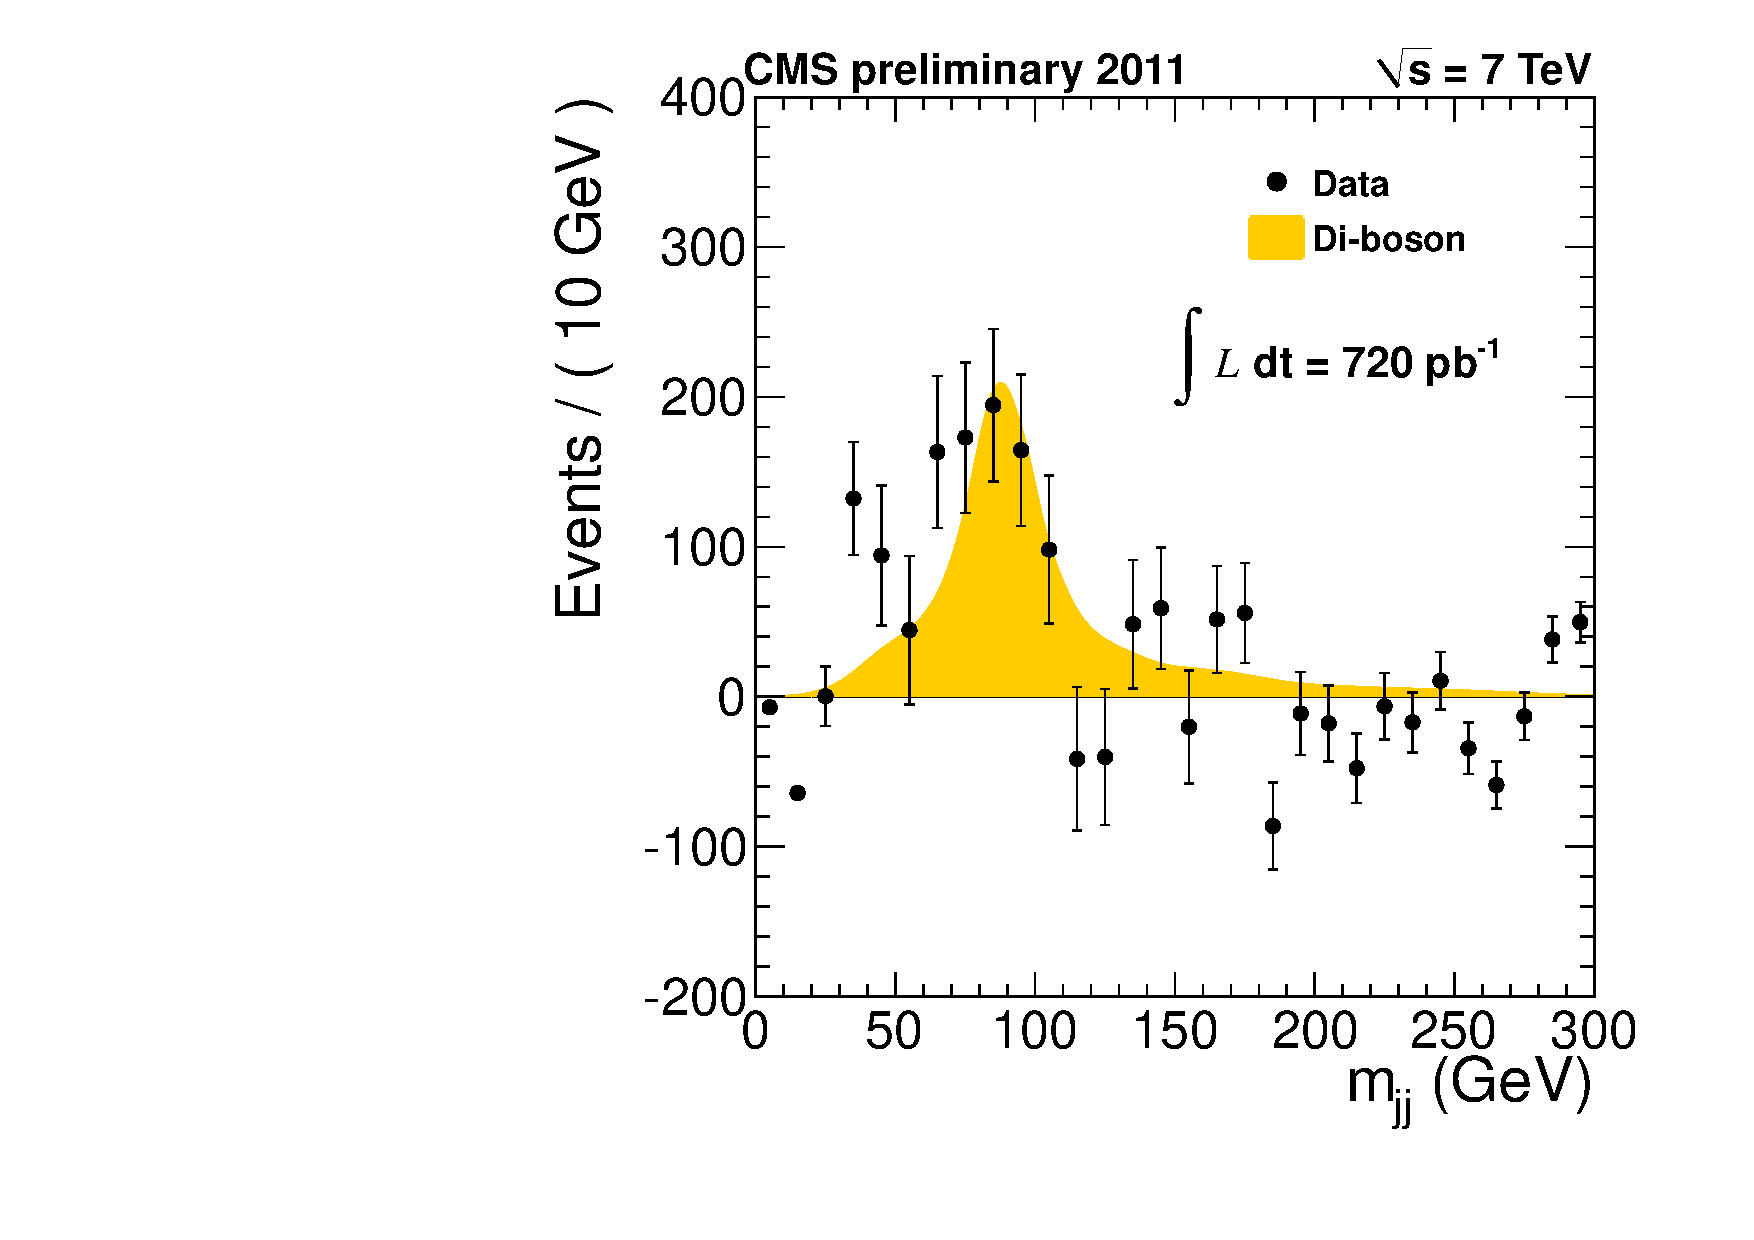
\includegraphics[width=0.5\textwidth]{figs/mJJ-combined-fit-subtracted.pdf}
    \caption{The dijet invariant mass distribution for the sum of 
      electron and muon events after subtraction of fitted 
      background components obtained in Figure~\ref{fig:CombinedFit}.}
    \label{fig:CombinedFitSubtracted}}
\end{figure}
%%%%%%%
%%%%%%%%%%%%%%%%%%%%%%%%%%%%
%%%%%%%%%%%%%%%%%%%%%%%%%%%%
%%%%%%%
\begin{figure}[h!] {\centering
\unitlength=0.33\linewidth
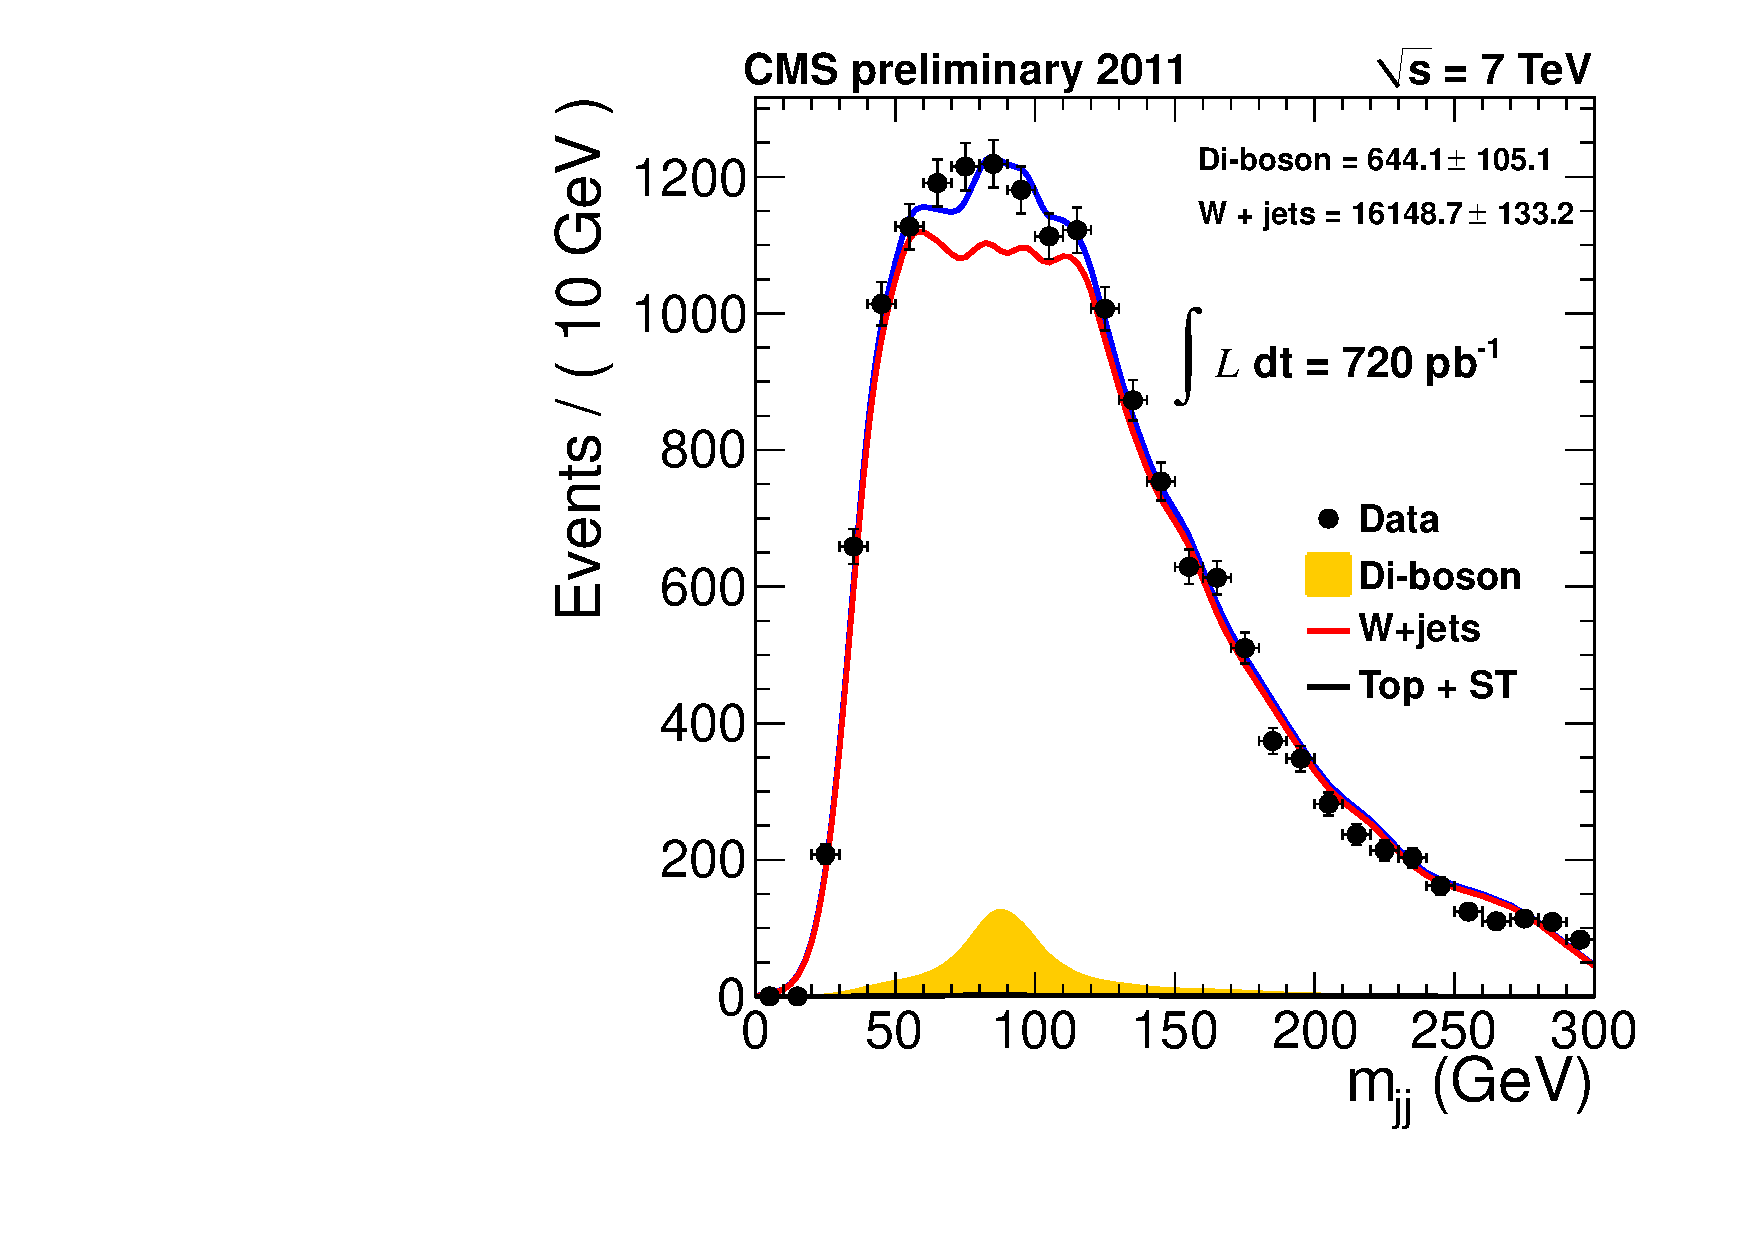
\includegraphics[width=0.48\textwidth]{figs/mJJ-mu-fit.pdf}
\put(-0.80,0.0){(a)} 
\unitlength=0.33\linewidth
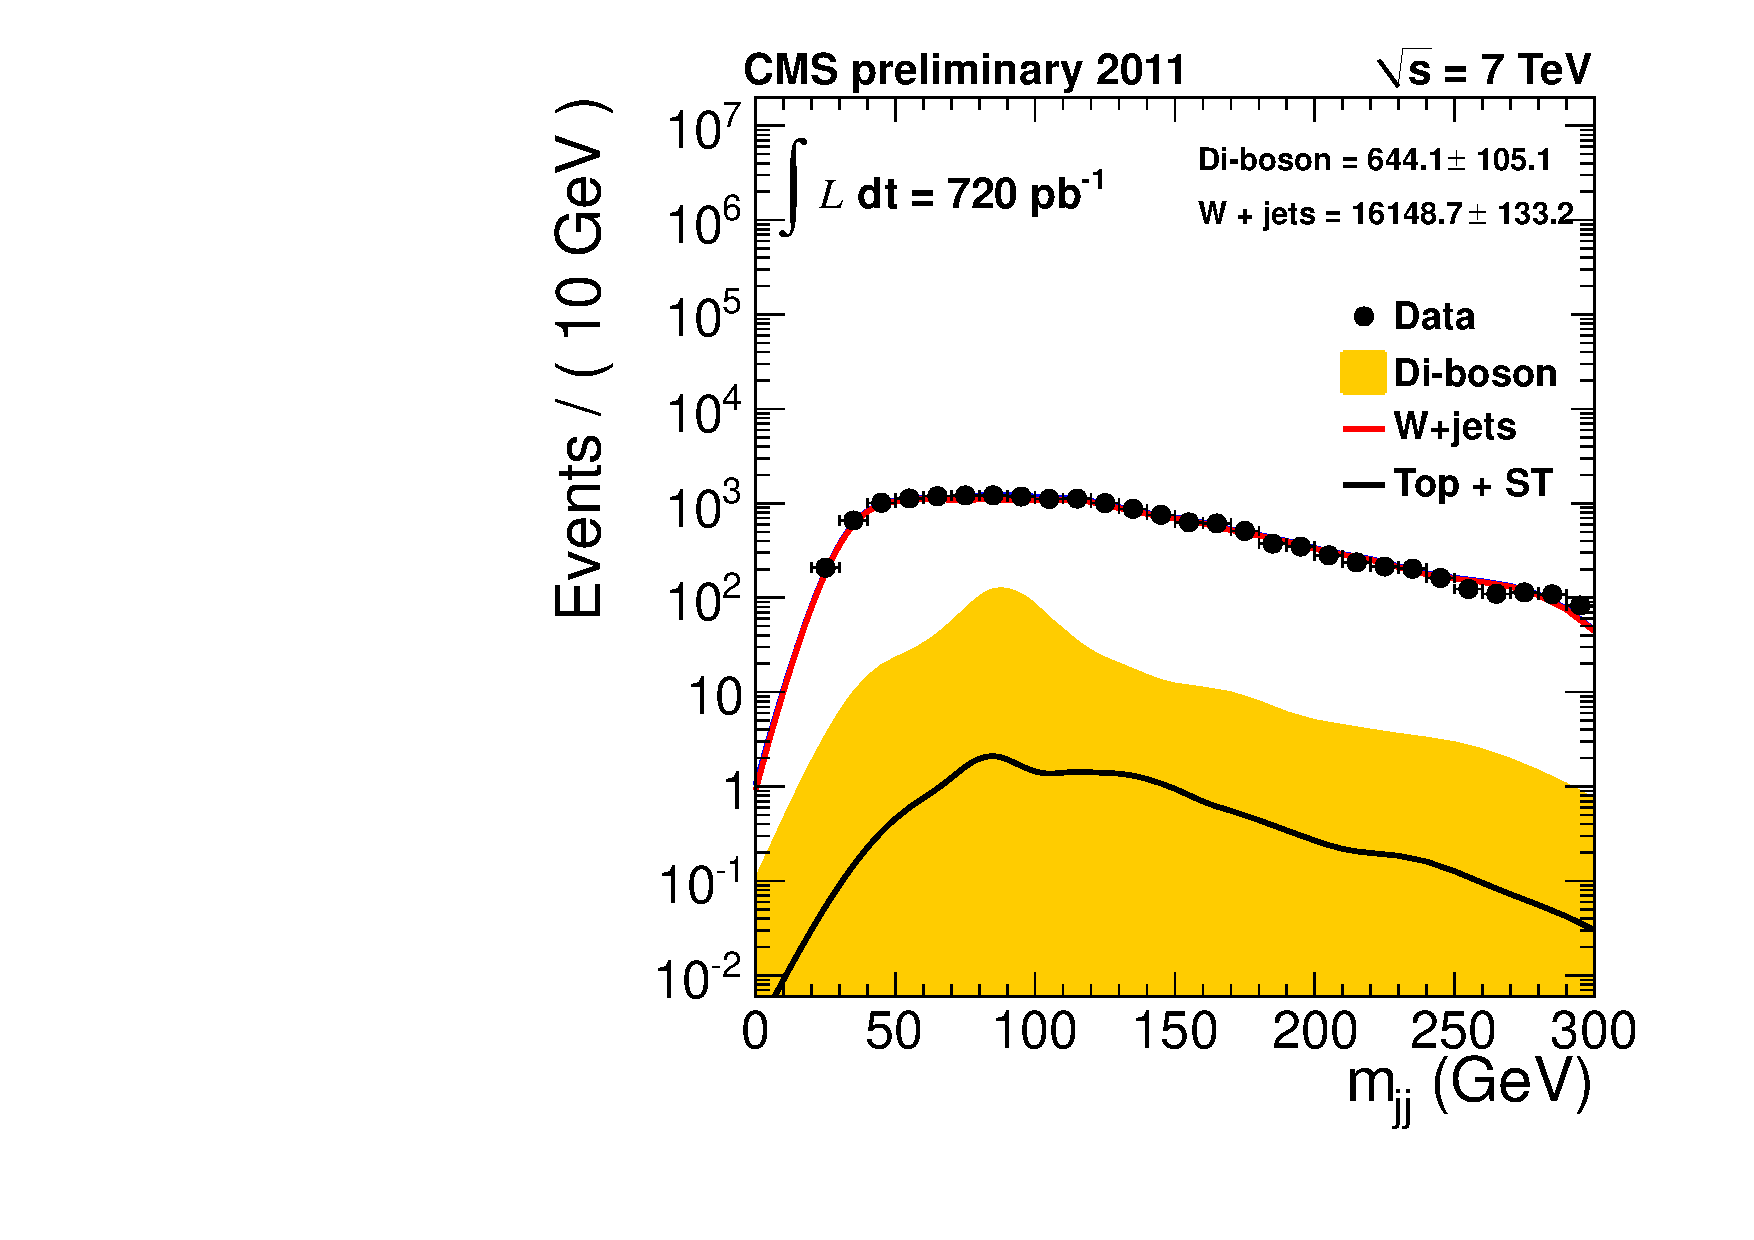
\includegraphics[width=0.48\textwidth]{figs/mJJ-mu-fit-logY.pdf}
\put(-0.80,0.0){(b)} 
\caption{
Projection of the $m_{jj}$ fit  to extract diboson signal for the muon 
data sample  (a) on linear scale and 
(b) on logarithmic scale.} 
\label{fig:MuFit}}
\end{figure}
%%%%%%%
%%%%%%%
\begin{figure}[h!] {\centering
    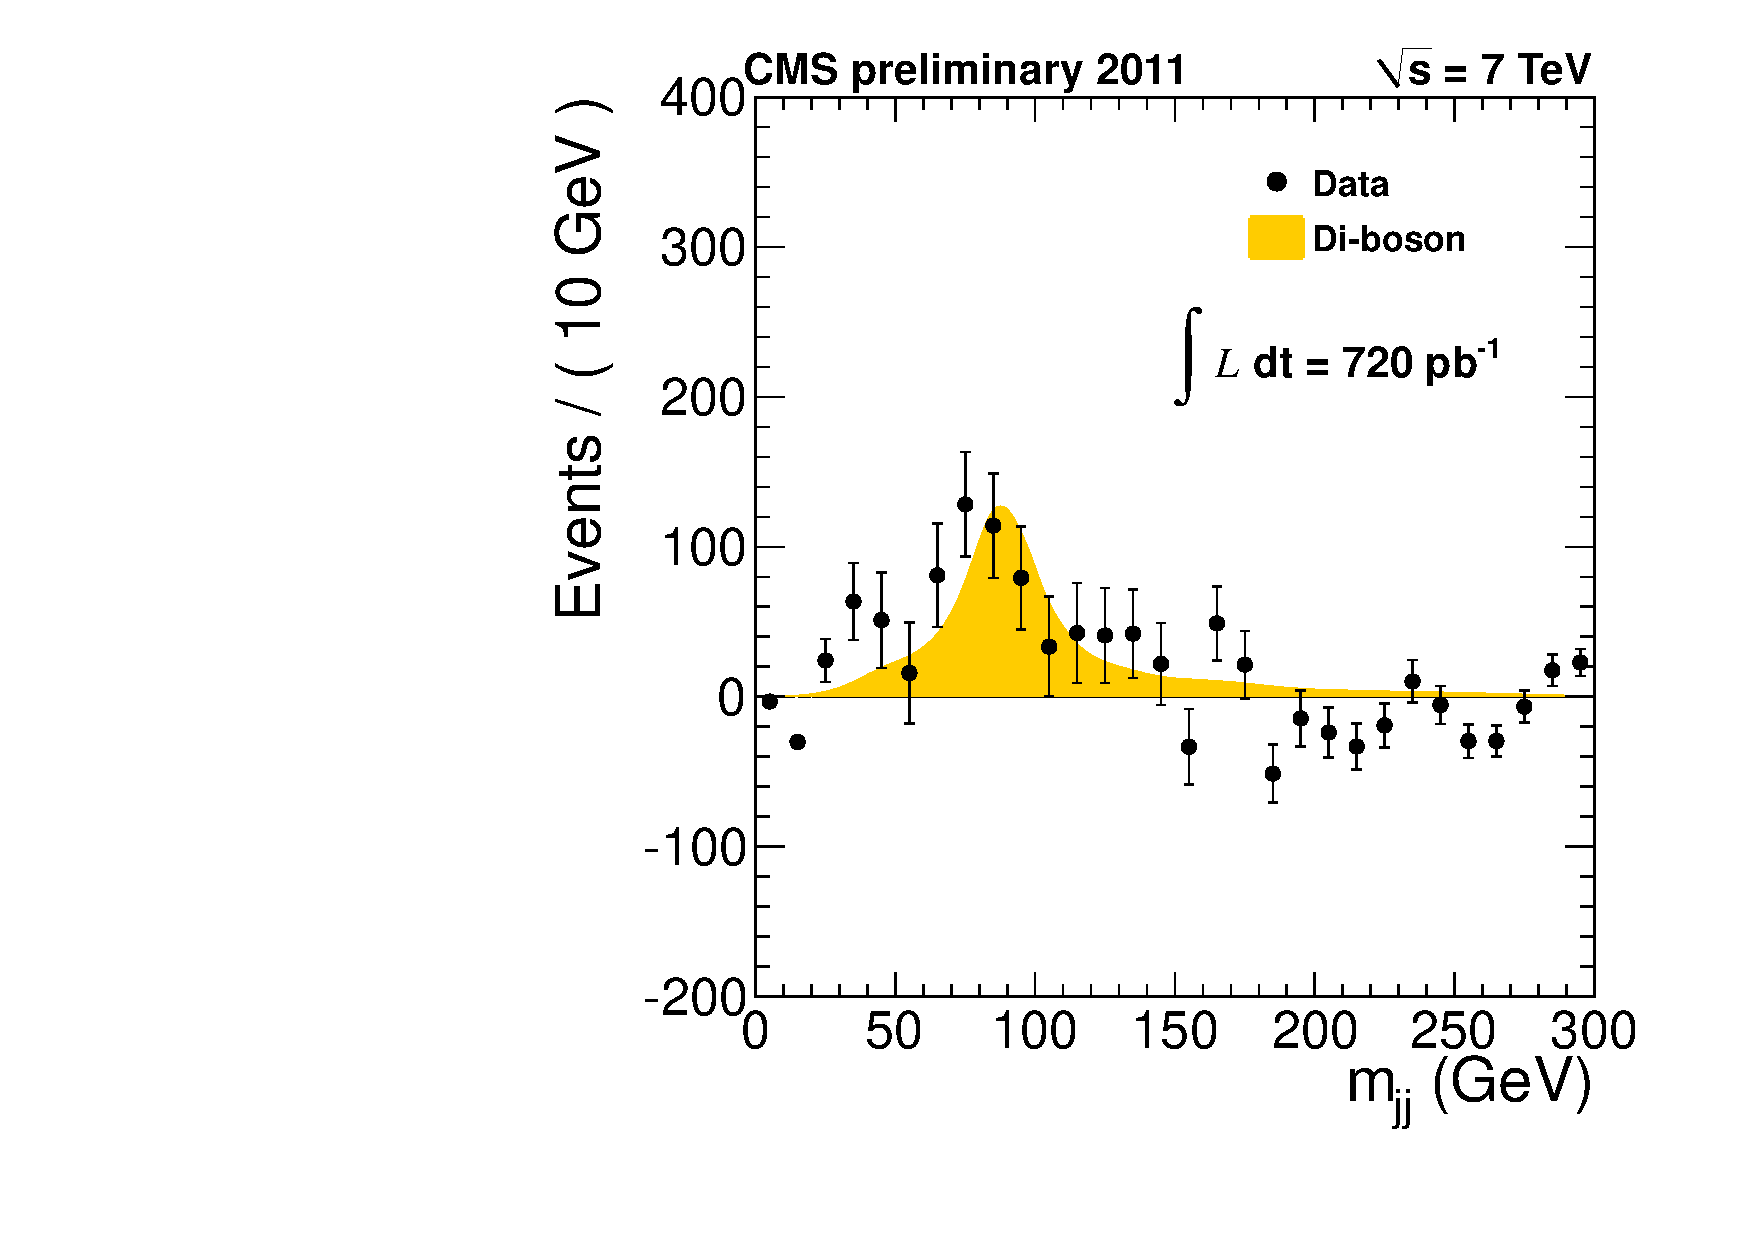
\includegraphics[width=0.5\textwidth]{figs/mJJ-mu-fit-subtracted.pdf}
    \caption{The dijet invariant mass distribution for the  
      muon events after subtraction of fitted 
      background components obtained in Figure~\ref{fig:MuFit}.}
    \label{fig:MuFitSubtracted}}
\end{figure}
%%%%%%%

%%%%%%%%%%%%%%%%%%%%%%%%%%%%
%%%%%%%%%%%%%%%%%%%%%%%%%%%%
%%%%%%%
\begin{figure}[h!] {\centering
\unitlength=0.33\linewidth
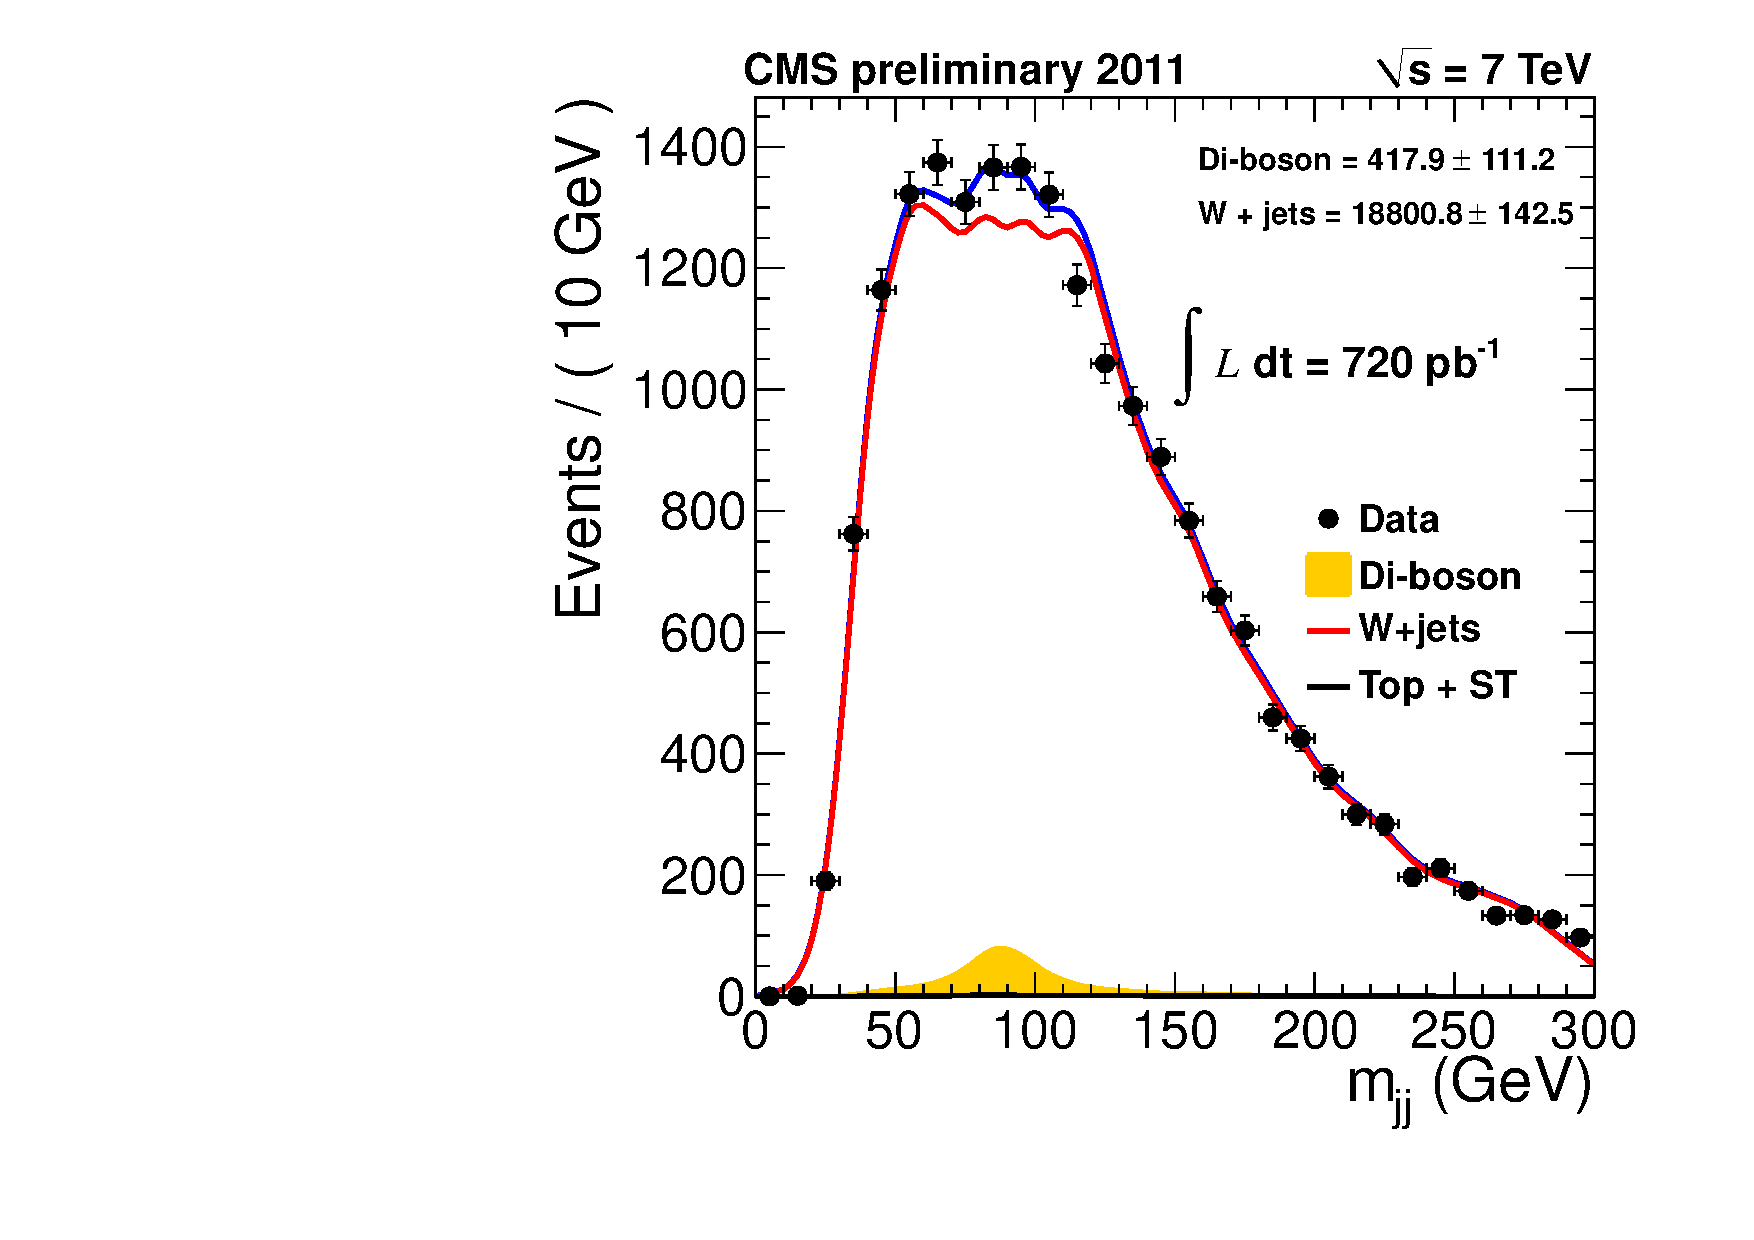
\includegraphics[width=0.48\textwidth]{figs/mJJ-ele-fit.pdf}
\put(-0.80,0.0){(a)} 
\unitlength=0.33\linewidth
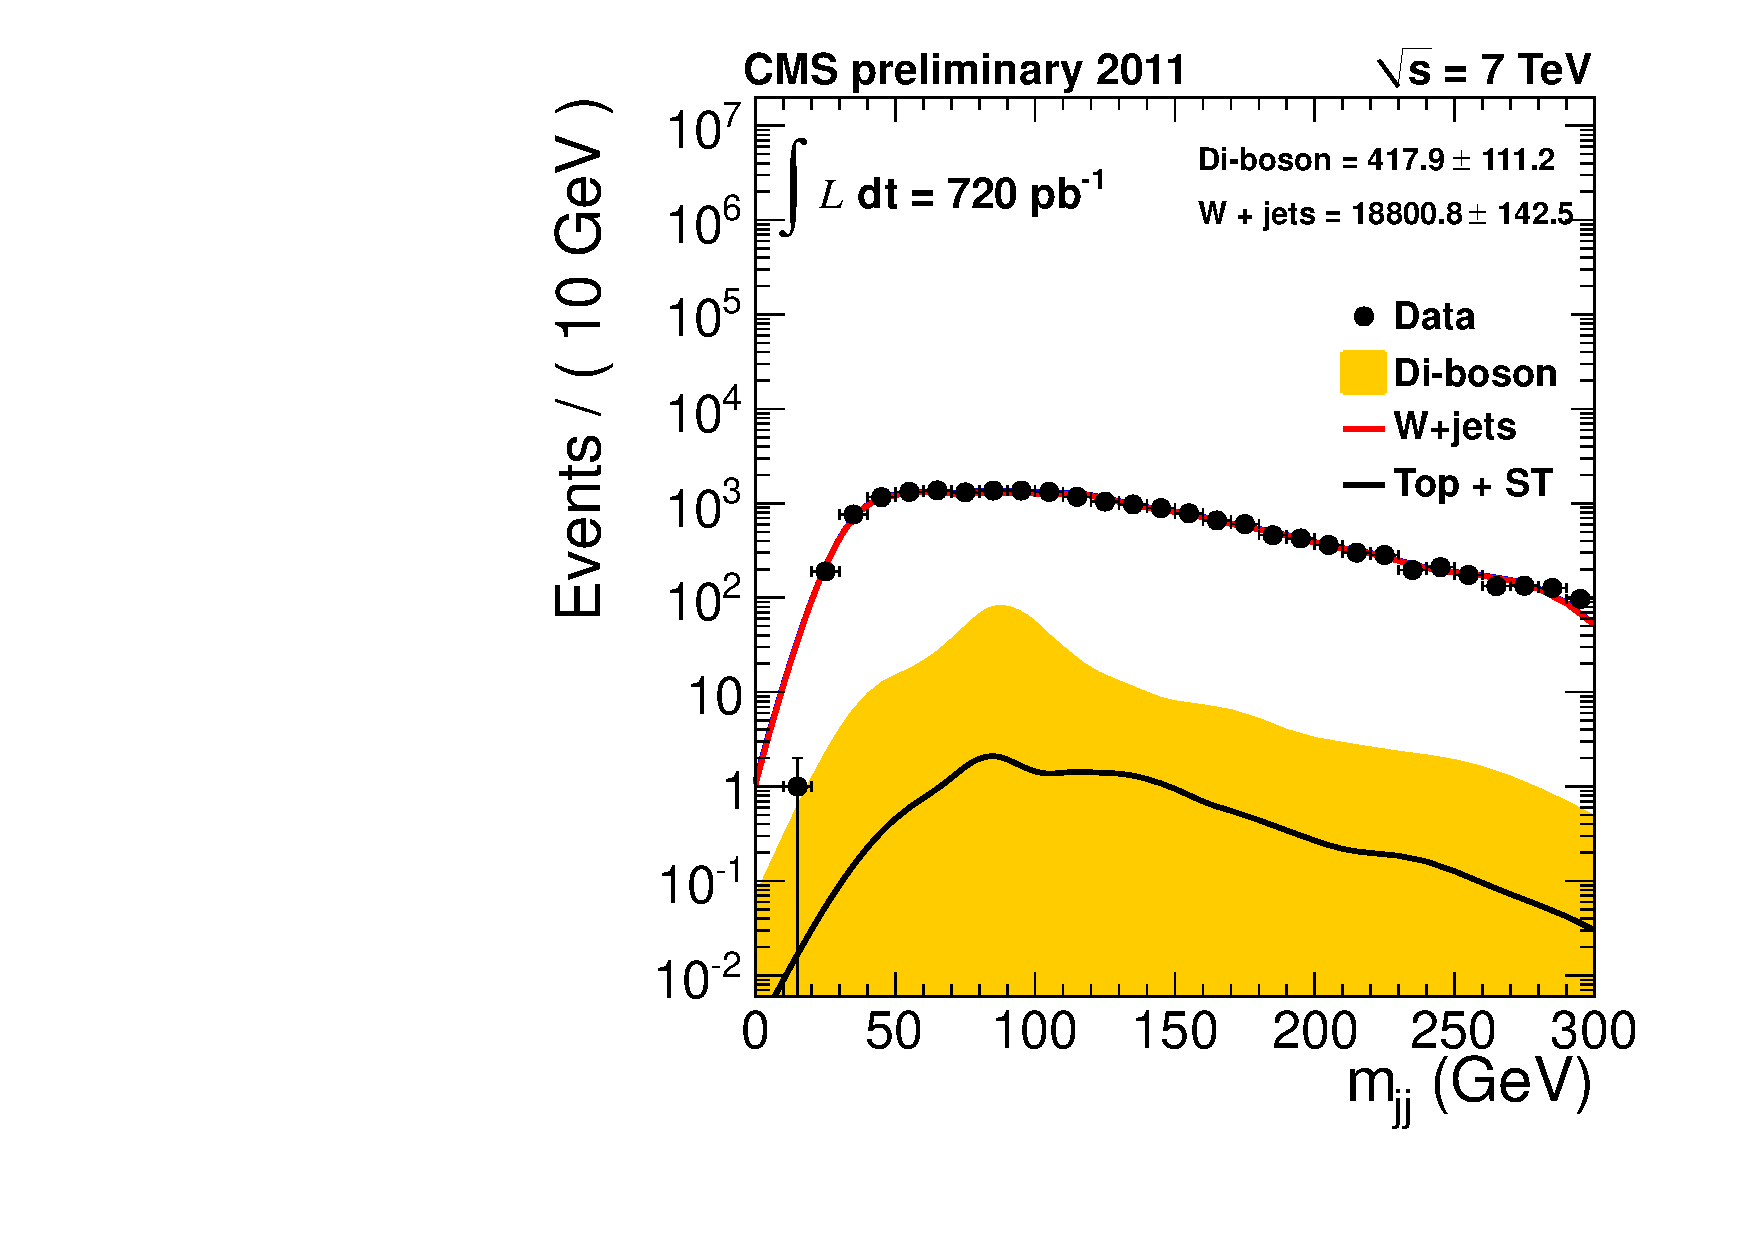
\includegraphics[width=0.48\textwidth]{figs/mJJ-ele-fit-logY.pdf}
\put(-0.80,0.0){(b)} 
\caption{
Projection of the $m_{jj}$ fit  to extract diboson signal for the electron 
data sample  (a) on linear scale and 
(b) on logarithmic scale.} 
\label{fig:EleFit}}
\end{figure}
%%%%%%%
%%%%%%%
\begin{figure}[h!] {\centering
    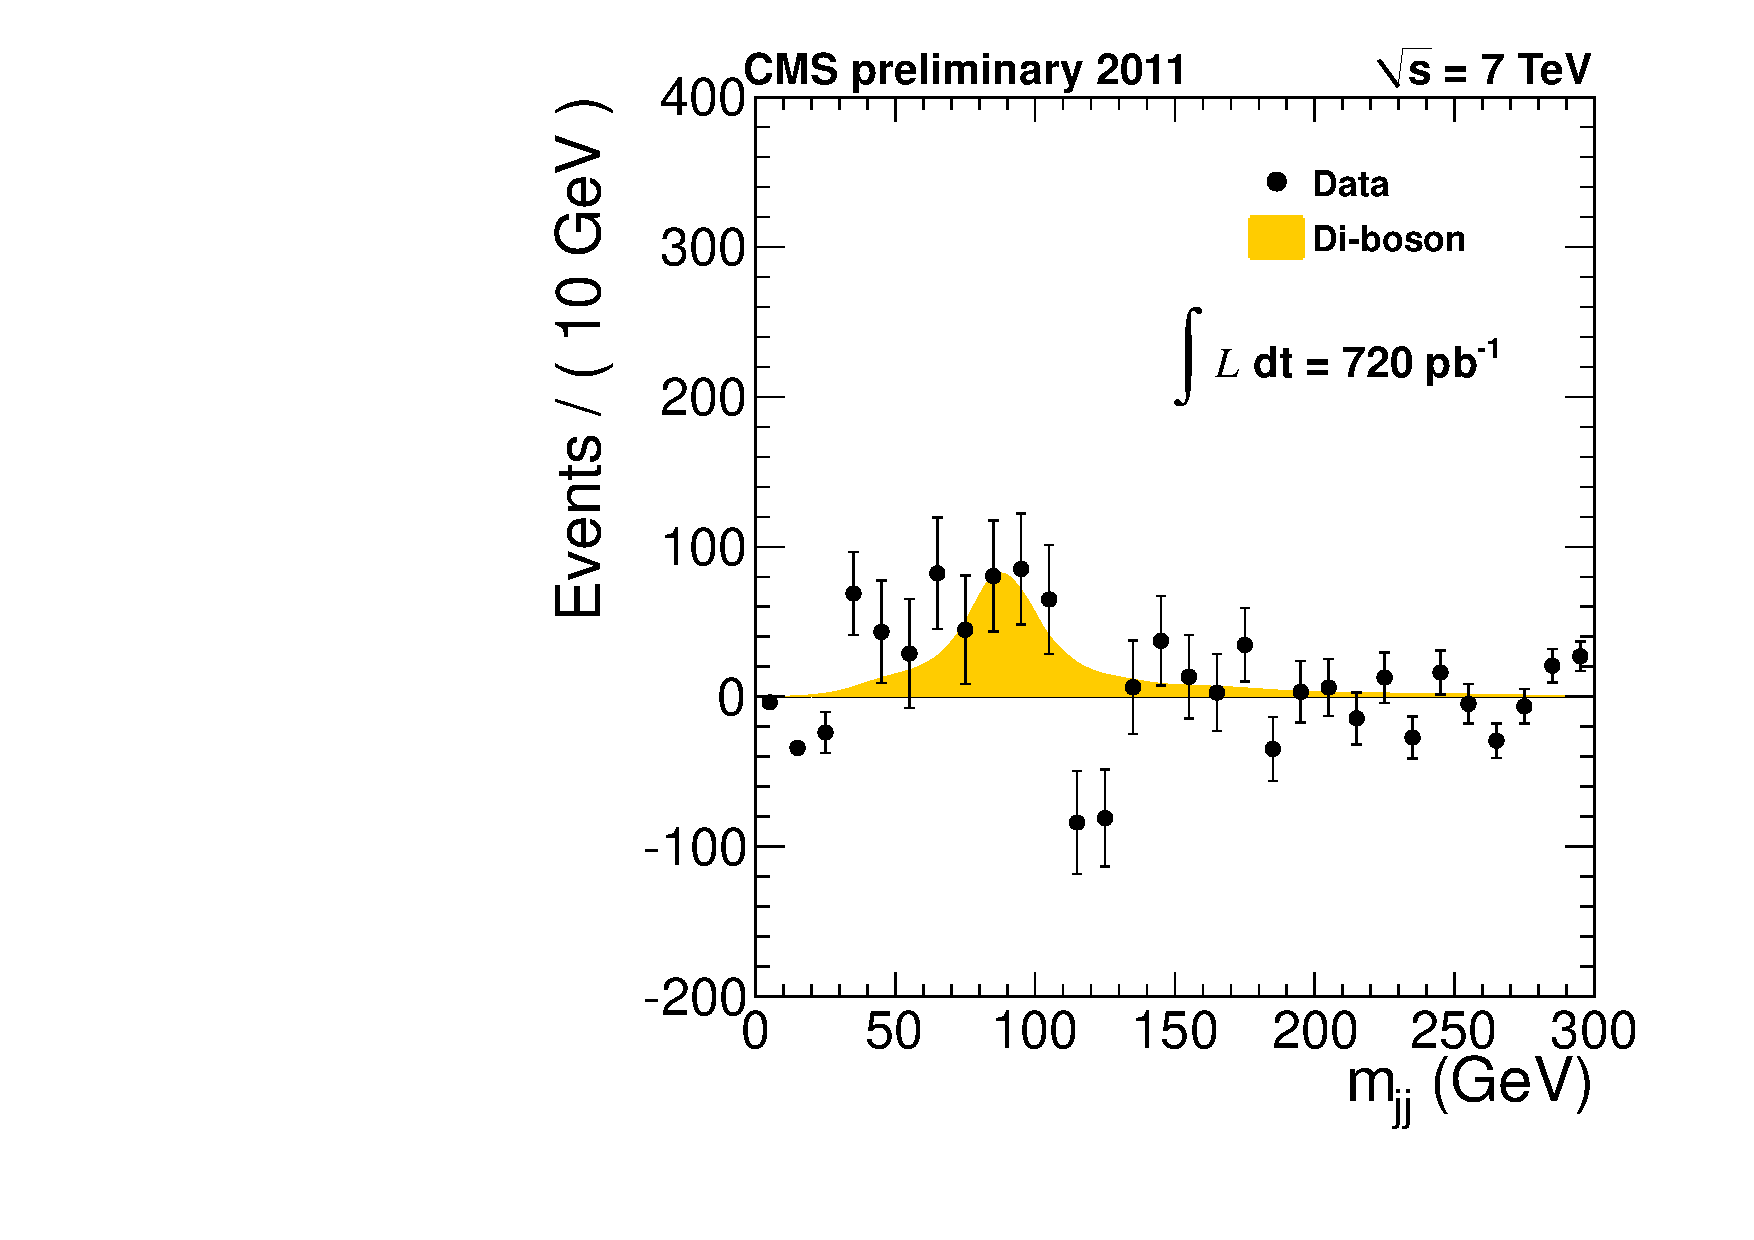
\includegraphics[width=0.5\textwidth]{figs/mJJ-ele-fit-subtracted.pdf}
    \caption{The dijet invariant mass distribution for the  
      electron events after subtraction of fitted 
      background components obtained in Figure~\ref{fig:EleFit}.}
    \label{fig:EleFitSubtracted}}
\end{figure}
%%%%%%%
